
\withsectionpage
\section{LoRaWAN (MAC-Layer)}

\begin{frame}{LoRaWAN Topology}
\alert{LoRaWAN} ist eine Abkürzung für \alert{Long Range Wide Area Network}\\
und wird von der \href{https://lora-alliance.org/}{\alert{LoRa Alliance}} standardisiert.

  \begin{center}
    
\includegraphics[width=0.28\textwidth]{material/lorawan-logo.png}\\
    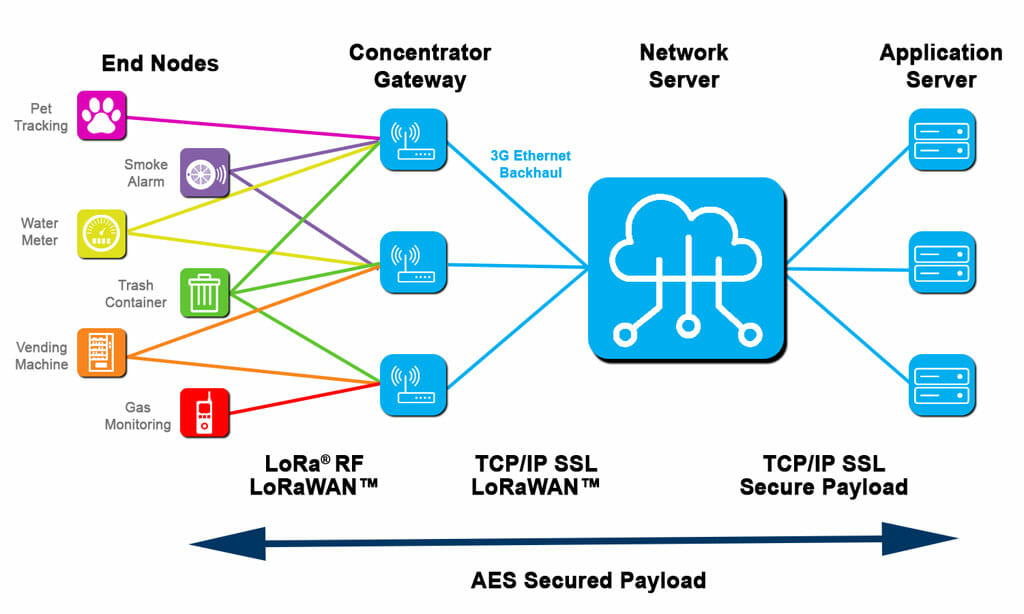
\includegraphics[width=0.5\textwidth]{material/lorawan-topography.jpg}
  \end{center}
\end{frame}
